% MAINTAINED F095 APPENDIX. Numeric tables originate from
% experiments/f095_campaign/gen_app_tables.py, but audited wording in this
% file is maintained separately. The generator writes the reproducible
% reference app_f095_generated.tex and does not overwrite this file.
\section{f095 Follow-up: Capacity, Symmetry, and Decomposition}
\label{sec:f095}
Unless noted, cells use the same dev E bank ($n_{quartet}{=}237$, $n_{parent}{=}106$), with training seeds 11/23/47; seeds and model arms are not independent datasets. checkpoints, banks, and manifests are in \texttt{artifacts/f095\_campaign/}.
\paragraph{Three-part decomposition.} With per-quartet scores for states A/B/AB, $1-J$ splits into per-case unorderability, no-common-threshold incompatibility, and working-point gap (Fig.~\ref{fig:u03}). Representation (raw$\to$relational) collapses the first segment; flip coverage on relational input collapses the third; incompatibility is the largest segment in every arm.
The split replicates on the order-free D03-E bank ($n{=}1838$ quartets, parents unseen by N models): ordering/incompatibility/working-point segments for raw+flip (0.122/0.648/0.016, 0.179/0.637/0.019, 0.154/0.636/0.053); rel+flip (0.024/0.322/0.051, 0.023/0.275/0.051, 0.020/0.281/0.050) --- same structure as dev512, so the decomposition is not bank-specific.
\begin{figure}[t]
\centering
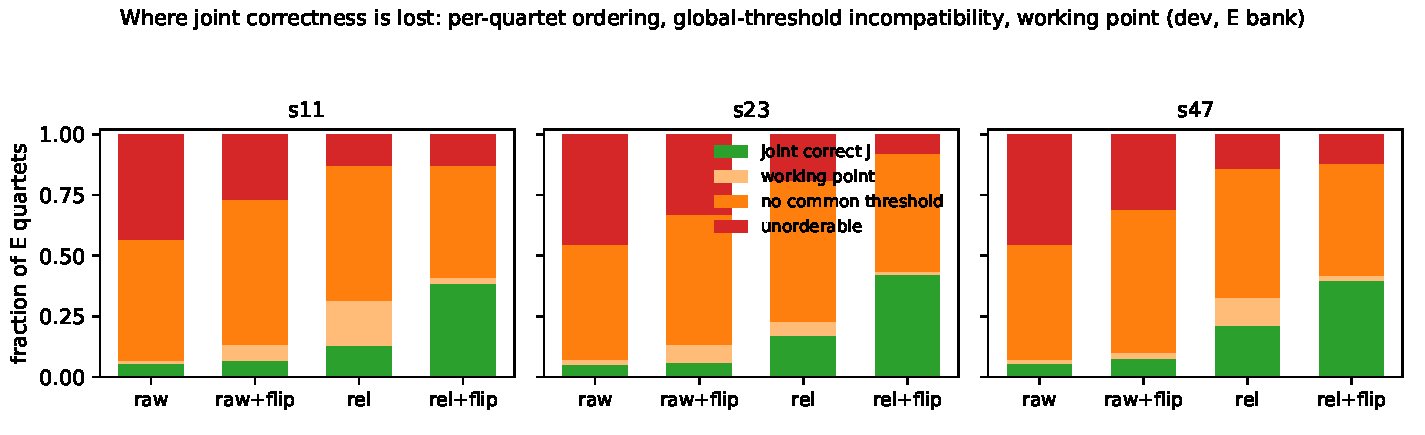
\includegraphics[width=0.95\linewidth]{figures/figU03_decomp.pdf}
\caption{Where joint correctness is lost on the dev E bank (237 quartets, 106 parents): stacked \(1-J\) decomposition per arm and seed. Green is joint-correct J.}
\label{fig:u03}
\end{figure}
\paragraph{Capacity and data frontier (D01, clean arm).} Under the tested recipe, $44\times$ parameters do not improve J; $16\times$ data lifts both arms but does not close the representation gap (Table~\ref{tab:d01}). Flip-BCE runs collapsed in 6/12 cells (flat loss, \(J{=}S{=}0\)); all 6 collapsed cells remain reported; capacity and optimization are not excluded.
\begin{table}[t]
\centering
\small
\begin{tabular}{@{}llll@{}}
\toprule
Cell & params & $J$ (s11/s23/s47) & $S$ \\
\midrule
% w64$\times$N (anchor): .055/.051/.055; w256$\times$N: .025/.046/.038; w512$\times$N: .059/.038/.029; w256$\times$4N: .110/.139/.084; w256$\times$16N: .148/.186/.173
w64$\times$N (anchor) & 6.8k & .055/.051/.055 & .565/.544/.544 \\
w256$\times$N & 84.6k & .025/.046/.038 & .582/.587/.582 \\
w512$\times$N & 300k & .059/.038/.029 & .557/.540/.485 \\
w256$\times$4N & 84.6k & .110/.139/.084 & .688/.709/.722 \\
w256$\times$16N & 84.6k & .148/.186/.173 & .827/.840/.844 \\
\bottomrule
\end{tabular}
\caption{D01 clean-arm frontier. Width cells share train\_101; data cells nest N$\subset$4N$\subset$16N. Full per-seed table with atomic/S/J* in the run JSONs.}
\label{tab:d01}
\end{table}
\paragraph{Symmetry control (D02) and structural follow-ups (U01/U02).} Group-averaging the 8 legal relabelings (same checkpoint, $8\times$ forwards) improves several arms but leaves errors (Table~\ref{tab:d02}); the source-task invariant typed-pair net is worse than raw under this recipe. That negative does not exclude learnable relational ability: its segment-sum plus linear readout cannot represent a general crossing (\texttt{artifacts/e832\_focus/structure/EXPRESSIVITY\_REPO\_AUDIT.json}). We do not claim a repaired model succeeds on the bank. TypedTri and TypedDisk use a different fusion and are not covered by that witness. Six distances reproduce the relational gain and a depth-matched concatenation does not under this recipe. This does not isolate geometry from optimization.
\begin{table}[t]
\centering
\small
\begin{tabular}{@{}lllll@{}}
\toprule
Arm & $J_{\mathrm{ident}}$ & $J_{\mathrm{avg}}$ & per-\(g\) range & all-8 raw \\
\midrule
raw & .055/.051/.055 & .038/.055/.055 & [0.021,0.110] & .000/.000/.000 \\
raw+flip & .068/.059/.076 & .152/.055/.118 & [0.046,0.114] & .000/.000/.000 \\
rel & .131/.169/.211 & .114/.105/.114 & [0.118,0.211] & .004/.000/.029 \\
rel+flip & .384/.422/.397 & .506/.515/.452 & [0.350,0.494] & .122/.089/.068 \\
typed clean/flip & .013/.025/.008 & .017/.008/.017 & --- & --- \\
sixdist clean/flip & .122/.173/.194 & .439/.426/.253 & --- & --- \\
concat clean/flip & .034/.025/.034 & .059/.084/.046 & --- & --- \\
g8-aug clean/flip & .076/.194/.080 & .363/.308/.245 & --- & --- \\
\bottomrule
\end{tabular}
\caption{Symmetry and structure: group-averaged vs identity J (top, D02); all-8 refers to the original model, not the averaged model. Exact group averaging makes its all-orbit accuracy equal to its identity J. Typed-pair, six-distance, and concatenation follow-ups (middle, U01/U02); symmetry-augmented training (bottom, D02-aug: identity J, disagreement stays .46--.76). s47 sixdist-flip is under-converged (noted, not load-bearing).}
\label{tab:d02}
\end{table}
\paragraph{Representation versus optimization: warm-start, protection and optimizer family (O01).} On a new-parent pool (1,229 quartets, 250 eligible parents) with the same clean starting weights and the same 300 full-batch steps, pairwise-distance input exceeds raw coordinates by $\Delta J=+0.434$ to $+0.561$ across 18 equal-recipe pairs (N and 4N, three seeds, three learning rates; every parent-clustered interval excludes zero), and the advantage survives a wider optimizer family (SGD momentum at two rates plus Adam at $5\times10^{-4}$ for 600 steps, selected on development BCE): $+0.475$ to $+0.574$ from both warm and scratch starts. The two input regimes are disjoint once the disclosed collapsed configuration is set aside. Across the full 648-configuration sweep the best raw $J$ at full flip coverage is $0.168$ (N) and $0.345$ (4N), and distance arms reach as low as $0.011$; every arm at that floor is an SGD-momentum-$0.003$ run from scratch, and all twelve full-dose arms below $0.05$ belong to that one configuration. Excluding it, the worst distance $J$ is $0.542$ (N) and $0.583$ (4N), still above the best raw value; within the main factorial (both starts, plain training, 36 arms per input and size) the ranges are fully disjoint --- distance $[0.562,0.697]$ (N) and $[0.737,0.856]$ (4N) against raw $[0.120,0.167]$ (N) and $[0.196,0.309]$ (4N). Retained-label efficiency is large but supervision-side only: distance models with 25\% of the retained change labels exceed raw models with 100\% ($\Delta J=+0.378$ to $+0.542$), and 88--96\% of the total distance gain is already present at 25\%, while mining cost is dose-independent (N 147,514 and 4N 587,320 candidate queries for all doses). Continuing from a clean checkpoint into flip training is \emph{not} better than training with flip data from the start ($-0.081$ to $-0.024$ at full coverage; $\approx0$ at zero dose), which rules out the reading that a clean model simply needs to be continued. Protection-style and replay losses buy forgetting-resistance rather than accuracy: their $J$ difference from plain continuation is at most $0.053$ in absolute value while they reduce the rate at which initially correct atoms become wrong on unseen parents by 4--12 percentage points, and the balanced preserve/flip arm achieves this with half the change labels. The J-scale interaction is positive with an interval excluding zero in 22 of 24 cell$\times$dose$\times$start combinations, the exceptions being two seeds at 4N/scratch/full dose. Two caveats bound this: raw is not shown to be at its capacity limit (13 of 72 warm full-dose raw arms have training error above 5\%, and parameter counts are not matched), and the 25\% and 100\% levels are retention amounts on one pool rather than two independent test sets, so the result is not a saving in oracle queries or annotation cost.
\paragraph{Coverage response (U07, supported on direction).} 25\%-flip coverage on six-distance exceeds raw at 100\% on both pools (6/6 pool--seed cells; Table~\ref{tab:u07}); on raw, more flip data helps but stays below six at a quarter of the retained flip pool under the tested recipe. Both arms use the same mined pool; this measures retained-example efficiency, not oracle-query savings.
\begin{table}[t]
\centering
\footnotesize
\setlength{\tabcolsep}{3pt}
\begin{tabular}{@{}lllllll@{}}
\toprule
 & N clean & N 25\% & N 100\% & 4N clean & 4N 25\% & 4N 100\% \\
\midrule
raw & .055/.051/.055 & .072/.034/.034 & .068/.059/.076 & .110/.139/.084 & .076/.160/.000 & .228/.279/.236 \\
six & .122/.173/.194 & .270/.321/.350 & .439/.426/.253 & .388/.359/.308 & .443/.460/.439 & .561/.540/.565 \\
\bottomrule
\end{tabular}
\caption{U07 coverage response (dev J). Raw-4N 100\% cells are dedicated flipmine-only reruns: they converge (J .23--.28). Earlier joint-run collapses remain historical outcomes; RNG causation has not been established. Six-25\% exceeds raw-100\% on both pools, 6/6 pool--seed cells.}
\label{tab:u07}
\end{table}
\paragraph{Football geometry (D06, historical single-edit probe).} On 721 real WOY passes, at least one keep and one flip edit within the assumed motion cap exist in 3.0\% at event time (3.2\% successful, 2.5\% unsuccessful) and 3.3\% 1.5\,s before; contested subpopulation (margin$<1$, n=278) 7.2\%. These are single-edit support rates, not E-quartet rates: no A/B/AB joint condition was tested. They do not establish football infeasibility or close natural/partial-observation routes. The zone-crossing anchor is unaffected. The old \texttt{paired} statistic (``at least one keep and one flip'') is reported as \texttt{supported\_single\_keep\_and\_flip} and reproduces field by field on the 721 WOY passes ($22/721=3.05\%$).
\paragraph{Natural E occurrence rate on real tracking (R08).} From 240 sampled real pass events, 162 pass the role/timestamp audit and supply 1,449 legal candidate situations. Using each candidate's and its t1-time constraining defender's \emph{real} subsequent displacement within the 0.2\,s motion cap ($1.214/1.199/1.174$\,m per match) with the passer and the other ten defenders fixed gives 7,117 qualifying real frame pairs. The full E quartet ($y(x{+}e_A)=y(x{+}e_B)=y(x)$ and $y(x{+}e_A{+}e_B)\neq y(x)$) holds for only $10/7{,}117$ frame pairs ($5/2{,}821$, $1/3{,}053$, $4/1{,}243$), i.e.\ a situation-level natural rate of $8/1{,}449=0.55\%$ ($0.70\%$, $0.16\%$, $1.18\%$ per match; event-cluster intervals $0.17$--$1.41\%$, $0.00$--$0.49\%$, $0.00$--$2.41\%$) and an event-level rate of $8/162=4.94\%$. On the same 1,449 situations, controlled within-cap search finds a witness in $670/1{,}449=46.2\%$, so search constructibility overstates natural occurrence by about $84\times$ ($63\times/282\times/45\times$ per match). Conditional on both single edits preserving the base label, the search rate is $5{,}066/216{,}924=2.34\%$ against a natural rate of $10/6{,}485=0.15\%$. The natural rate rises monotonically with the observation window: $0.55\%$ at $0.2$\,s, $4.55\%$ at $0.4$\,s, $11.94\%$ at $1.0$\,s and $16.98\%$ at $2.0$\,s, so any statement about how common E is must name the window. On actually selected receivers the $0.2$\,s rate is $0/155$ (rising to $5/155$, $14/155$, $25/155$ at $0.4$, $1.0$ and $2.0$\,s), too few to test any preference. As a real-frame control, within $0.2$\,s the channel label genuinely flips in $260/7{,}117=3.65\%$ of pairs, but substituting the t2 whole-frame real coordinates leaves only $4/7{,}117=0.06\%$ satisfying E. No threshold is used to declare infeasibility: E does occur in real data, so it is reported as a rare stress test, its labels come from a model-independent geometric oracle rather than pass success, and the joint cell is a crossing of two real single-player displacements rather than an observed frame.
\paragraph{Fresh-bank confirmation (D09, confirmed).} On the archived 236-quartet bank, six-distance beats raw by +0.259/+0.364/+0.195 (flip) and +0.106/+0.072/+0.178 (clean): 6/6 frozen predictions hit. An old integer-ID audit excluded 18 quartets; this namespace-based filter was erroneous. That correction does not revive an integer-ID leakage charge against \texttt{dev512}. Historically, excluding them (n=218) retained the advantage (gaps +.26/+.37/+.22 flip, +.10/+.07/+.18 clean), but this is not a deduplicated result. D03-E ($n{=}1838$) also reproduces the ordering for N models. Its parents are not fresh for every 4N/16N model. Freshness is checkpoint-specific; these are reanalyses, not new sealed confirmations.
\paragraph{Flip-loss weight (LAM, negative-for-cause).} $\lambda\in\{0.25,0.5,2.0\}$ gives J .042/.080/.089 / .068/.084/.059 / .080/.105/.063, under this limited sweep: this sweep does not identify the cause of large-scale collapse; g8 augmentation recovered 6/6 tested cells.
\paragraph{Vision input-scale$\times$init factorial (D04).} ResNet-18 \citep{he2016deep} on rendered quartets, ImageNet-pretrained \citep{deng2009imagenet} versus random init, joint consistency $J$ (pretrained $|$ random), seeds s803/s805/s806: 64px: .353/.367/.272 $|$ .177/.174/.104; 96px: .517/.501/.547 $|$ .064/.431/.366; 128px: .676/.669/.602 $|$ .040/.563/.450; 224px: .720/.737/.709 $|$ .000/.662/.611; head-only with historical BN adaptation at 224px: .221/.225/.232. All inputs are bilinear resizes of the same 64px image, so larger input adds no observation information. At 224px pretrained-minus-random gains are +72.03/+7.49/+9.87pp (mean +29.80pp, all seeds retained); pretraining equivalence is not established. The s803 random arm collapses at 128/224px, but its cause is unresolved. Historical head-only runs updated BN buffers and were not pure frozen probes. Without a static-only same-architecture arm, these results establish task competence, not a flip-repair effect.
\paragraph{Relation supervision to an image student (U06, historical recipe).} ResNet18 student, same images/labels: endpoint-only (A), +generic-geometry aux (B), +relation aux (C). J: A .353/.367/.272, B .296/.229/.212, C .285/.358/.278; shuffled-target sanity 0.249. At 224px the ordering repeats (A .720/.737/.709; B .691/.506/.713; C .691/.735/.687; shuffled .708/.673/.686): C does not improve A in these runs. Ordered endpoint targets can differ despite identical inputs from the renderer; exact indistinguishability is not assumed for every old-renderer orbit. Shuffled-target and training RNG were not isolated. These observations bound the old recipe and neither prove a noise-regularization mechanism nor rule out relation supervision.
\paragraph{Readout refit (U04, layer complementarity supported, narrowed).} Frozen-encoder refits (linear probes on frozen features \citep{kumar2022finetuning}) yield similar final-score ordering under the tested readouts (relflip static-readout S 0.8734/0.9198/0.8819); flip-readout gains appear on the static relational encoder (relfeat +0.059--0.160); the tested small-MLP adds <+0.021; broader nonlinear readouts remain untested. S is a property of the encoder-head composition, not of the encoder alone; flip readout on raw encoders only migrates errors (R\_full .05--.06, M .39--.48).
\paragraph{Prospective intervention test on a new task (O04).} To ask whether the $S$/$J$/$J^\ast$ decomposition can predict \emph{in advance} which segment an intervention moves, a prediction was written and sealed (hash recorded, written before any evaluation number) on the U10 tasks: T1, 2,724 E quartets from 322 parents; T2, 3,443 from 369. Readouts are refit on 512 new-task training scenes, with 409 fit parents and 103 head-dev parents, single-edit states following their parent. The pre-registered primary prediction (the intervention is attributed to the $J$ segment) holds in 7 of 8 cells, which we report as \emph{not supported} rather than relaxing the criterion to a majority; the secondary prediction that gains are not oracle-threshold movement ($|\Delta J^\ast|<|\Delta J|$) holds in 8/8 cells. Head-level change supervision helps only when the trunk itself never saw change supervision: T1 \texttt{six\_clean} $J$ rises $0.1946\to0.2841$ and T2 \texttt{six\_clean} $0.6952\to0.7441$, whereas already-flip trunks gain nothing ($\Delta J=-0.0115$ and $-0.0016$, with $J$ already $0.7483$/$0.9993$), and on raw trunks the same intervention is negative in 4/4 cells. Two further boundaries matter. First, a threshold chosen on dev can sit far below the oracle bound for the same score: T1 \texttt{six\_flip} with a static readout gives $J_{\text{dev}}=0.4574$ against $J^\ast=0.7905$ (T2: $0.8921$ vs $0.9995$), and change supervision can move the working point without moving the bound. Second, merely changing the readout feature parameterization from per-fit-parent standardization to whitening moves the segment attribution from 7/8 to 4/8 cells and changes the magnitude of the same intervention (T1 \texttt{six\_flip} $\Delta J$ from $-0.0115$ to $+0.3484$, with $J^\ast$ rising $+0.1396$ in step). Segment attribution and $S$ are therefore properties of $S(f_{\text{head}}\circ h)$, not of the encoder alone. This covers two tasks, two input parameterizations and MLP widths $\{16,64\}$; 77 of 96 candidates select their dev optimum at the final epoch, so the readout search is budget-capped, and the trunks and banks are reused f095 artifacts rather than a new confirmation. One structural limit deserves recording: the decomposition is defined only on cases carrying at least one positive and one negative state --- the production certificate raises on all-negative input --- so the $45.7$\% of decision scenes whose 49 candidates are all infeasible lie outside its domain of definition, and that share is a property of the candidate-feasibility contract rather than of any score. Feasibility is moreover shared by every candidate within a scene, so no per-candidate threshold can isolate infeasible scenes; only refusal can, which returns the question to the coverage axis. We therefore do not read the coverage collapse as evidence that the scores themselves are miscalibrated, since at a fixed budget the dev-selected threshold already sits within $0.0093$ net benefit of the oracle envelope.
\paragraph{Nearest-neighbor comparison (D08, training-path confound).} PCT-style continuation and scratch flipmine attain similar J (+0.008/-0.038/+0.000 on rel); balanced-half and random-half are within range on 2/3 and 1/3 seeds; temperature calibration moves no argmax decisions (24/24 cells), an algebraic identity, not a working-point exclusion. PCT starts from clean weights while flipmine starts from scratch, so this is not a loss-causal comparison. Balanced-half balances flip endpoint classes, not preserve/flip. Training-set regression cannot rule out unseen-parent regression or U05.
\paragraph{Decision policies (D10, historical incomplete enumeration).} For the archived dev-selected policy comparisons, flip-minus-clean is median +0.236/+0.105/+0.085 (historical intervals); these points are not a complete action frontier, and the old isotonic implementation was incorrect. Dev-matched coverage drifts on eval; these values do not establish equal eval coverage or exclude calibration.
\paragraph{Cross-task input advantage (U10).} T1 uses 2,724 E quartets from 322 parents; T2 3,443 from 369. P-A compares inputs under the same flip protocol: distance+flip exceeds raw+flip by +0.500/+0.563/+0.534/+0.392/+0.358/+0.356 (T1 then T2, three seeds each). P-B compares retained flip examples: distance-25\% exceeds raw-100\% in 6/6 cells. Neither test is an interaction test. The original J-scale interaction $I=(J_{distance+flip}-J_{distance})-(J_{raw+flip}-J_{raw})$ is T1 +0.3936/+0.4393/+0.4127; T2 -0.1891/-0.1719/-0.2503. T1 supports positive interaction; T2 is a negative-interaction boundary despite near-perfect combined J. T1 uses six pairwise distances; T2 uses three role-specified distances. The old typed P-C does not establish invariance because indexed normalization breaks exchangeability; corrected retraining is reported below.
Orbit averaging replicates cross-task: it lifts flip-trained arms (T1 six +0.062/+0.041/+0.090; T2 raw +0.069/+0.069/+0.067), 12/12 flip cells positive per task, has small clean-arm effects. Old typed changes below .01 do not demonstrate exact end-to-end invariance; that claim requires corrected preprocessing and retraining.
\paragraph{Collapse recovery (D08-six, cause unresolved).} A preserve-loss (pct) rerun on sixdist rescues the s47 collapse (J 0.376/0.439/0.452 vs flip-BCE .439/.426/.253; pct mean .422 vs flipmine .373). Continuation from clean and scratch training differ, so recovery cannot be attributed to the protection loss alone.
\paragraph{Decision frontier across encoders (D10-ext).} The historical dev-matched policy differences also occur for stronger encoders: rel12 median +0.449/+0.199/+0.217; sixdist median +0.208/+0.118/+0.315; positive-pair fraction .95--1.0 everywhere. These archived points retain the enumeration/calibration limitations above and require corrected policy analysis.
\paragraph{Full-universe deployment estimate (R09).} The corrected frontier is still conditioned on oracle-feasible scenes: of 256 scenes, 139 (54.3\%) admit at least one feasible candidate and 117 (45.7\%) admit none. Extrapolating a threshold selected on the 43 feasible dev scenes for target coverage $0.5$, with no feasibility filtering, to the remaining 213 scenes (117 of them infeasible, 54.9\% of that universe) gives measured coverage $0.1455$--$0.3239$ rather than dev's $0.4884$, i.e.\ 30--66\% of the target; in-action success is $0.2239$--$0.9459$ and per-scene net benefit $0.0322$--$0.1382$ (same-scene bootstrap intervals all positive over 213 scenes). These are extrapolations of a dev-matched policy, not an achieved equal coverage. At dev coverage budgets $0.25$ and $0.5$, relational encodings reject all 117 infeasible scenes ($0/117$, $0.0$\% of cost), whereas raw encodings act on $0$--$11$ and $4$--$25$ of them and spend $15.7$--$48.3$\% of total cost on scenes that cannot succeed; at budget $1.0$ the infeasible scenes absorb $14.8$--$93.0$\% of cost and per-scene net benefit spans $-0.033$ to $+0.189$ with five of six raw policies negative. Net benefit is an illustrative utility (one unit of success reward minus archived action cost) with no task-level validation, and at budget $0.5$ the flip-minus-clean net-benefit difference has no pair interval excluding zero (only in-action success does, in $4/9$ pairs); the sign turns favourable only at budgets $0.75$ and $1.0$ ($6/9$ and $5/9$), where thresholds are nested. Each model enumerates $24{,}966$--$31{,}311$ breakpoints collapsing to $1{,}700$--$1{,}934$ distinct action policies, so these are not independent repetitions, and intervals resample scenes only (2,000 draws). The oracle-label diagnostic envelope is an optimistic, selection-biased bound without valid intervals: at fixed coverage the dev-selected threshold lies within $0.0093$ net benefit of the same-coverage oracle point, and the unconstrained oracle optimum is driven mainly by coverage rather than threshold tuning. All of this reanalyses one fixed set of 256 scenes rather than confirming on new ones, and the dev scene set was itself selected by feasibility.
\paragraph{Readout refit on the order-free bank (U04-E).} The scoped P2 pattern replicates on D03-E ($n{=}1838$): flip-readout helps static relfeat encoders (s11 +0.045, 3/3 positive) but not already-flip-trained ones; static-S matches D03 values within .002 (float-level borderline quartets).
\subsection{Corrected pipeline and paired reanalysis}
These are repaired-pipeline runs and reanalyses of exposed banks, not new sealed confirmations. Four-arm intervals resample the same parent groups jointly (2,000 bootstrap draws). Small differences from historical I above arise from recomputing unrounded per-quartet outputs. One reproducibility caveat applies to the table below: floating-point reduction order depends on the thread count, and the two columns were produced under different settings. The $I$ column is computed from the raw/distance arms, whose historical checkpoints reproduce bit-exactly at four threads (36/36); the retrained typed models reproduce bit-exactly only at two threads (18/18), and the typed column reports that two-thread evaluation. The same typed flip arm can differ by up to 9.0pp between the two settings (T2, seed 11: $0.2495$ at four threads versus $0.3398$ at two), so the typed column must not be compared against typed numbers produced at another thread count; the raw/distance-derived $I$ is stable to within 2.2pp and is unaffected in sign or magnitude.
\begin{table}[t]\centering\small
\begin{tabular}{@{}llll@{}}\toprule
Task & Seed & $I$ [parent 95\% CI] & corrected typed+flip $J$ \\
\midrule
T1 & 11 & +0.3935 [+0.3410, +0.4453] & 0.2761 \\
T1 & 23 & +0.4394 [+0.3875, +0.4846] & 0.1780 \\
T1 & 47 & +0.4126 [+0.3607, +0.4600] & 0.2684 \\
T2 & 11 & -0.1891 [-0.2444, -0.1305] & 0.3398 \\
T2 & 23 & -0.1719 [-0.2232, -0.1177] & 0.3189 \\
T2 & 47 & -0.2504 [-0.3038, -0.1968] & 0.3404 \\
\bottomrule\end{tabular}
\caption{Corrected U10 analysis. T1: 2,724 quartets/322 parents; T2: 3,443/369. I uses the raw/distance clean/flip arms (four-thread reproduction). The typed column is a two-thread evaluation of models retrained with train-fitted role-shared normalization (18 runs: two tasks, three seeds, clean/25\%/full flip), the setting in which those checkpoints reproduce bit-exactly; it is not comparable to typed numbers computed at another thread count. Typed J remains below distance+flip under this recipe; this is not a parameter- or optimization-matched architecture proof.}\label{tab:u10fixed}\end{table}
\paragraph{Matched-capacity and matched-budget control for the typed comparison (O02).} The typed structure carries 39.5--46.3\% more parameters than raw/six ($9{,}553$ versus $6{,}529$--$6{,}849$), so its deficit could reflect optimization difficulty rather than representation. Shrinking it to $6{,}681$ parameters (within 2.5\% of raw/six) and re-evaluating all four arms on the same immutable pools does not close the gap: under an equal recipe, six+flip exceeds typed+flip by $+0.514/+0.529/+0.486$ (T1) and $+0.731/+0.701/+0.755$ (T2) across the three seeds, every parent-paired interval excluding zero, and selecting each arm's best recipe on the training objective alone (never on evaluation $J$) leaves $+0.499/+0.507/+0.505$ and $+0.645/+0.675/+0.667$. Shrinking typed does not help by itself (typed\_m minus typed\_o is $-0.038/+0.019/+0.016$ on T1 and $+0.017/-0.056/-0.091$ on T2). Training objectives show persistent fitting difficulty under these recipes, without isolating its cause: under the historical recipe typed's final training objective is $0.27$--$0.50$ (T1) and $0.25$--$0.26$ (T2) against $0.006$--$0.021$ and $3\times10^{-5}$--$10^{-3}$ for raw/six, and even after a tenfold budget increase with lower learning rates typed's best per-recipe mean is $0.0804$ (T1) and $0.00256$ (T2) against $3.3\times10^{-5}$ and $1.6\times10^{-6}$ for the best of raw/six, roughly $10^{3}$ times worse, while raw/six stay on their plateau ($J$ moves by at most $0.6$pp). The control covers one width and a budget ladder of three learning rates by two step counts, so it bounds this recipe family rather than the architecture in principle, and it matches parameter count but not parameter distribution or depth. This target-task comparison is not the source-task segment-sum witness, and it is not used to exclude learnable relational ability. These values refer to the original matched-budget run; a numerical-order repeat changes individual seed values while retaining the direction, and does not establish numerical identity.
\paragraph{Pipeline symmetry.} Saved/reloaded full pipelines give maximum logit differences T1: 21.54$\to$3.05e-05 (prediction differences 0); T2: 23.58$\to$0 (prediction differences 0). T1 residual is float summation tolerance; the old indexed statistics caused substantive differences. Corrected invariance is an engineering result, not an accuracy guarantee.
\paragraph{Visual observability audit.} On 512 training parents, 492/512 have identical images throughout the four within-color endpoint swaps; the other 20 exhibit rasterization differences (maximum pixel difference 0.80). Oracle labels are unchanged throughout. Thus ambiguous identical-image cases exist, but the old renderer is not globally exactly invariant. Orbit target variation cannot be equated with the actual old training loss or its sole failure cause. The repaired renderer sorts same-color endpoints without labels before rendering, yielding identical images for all 512 audited orbits. Subsequent visual comparisons use this changed observation protocol; their old/new absolute J values are not a matched repair effect. The completed canonical visual matrix is reported separately below.
\paragraph{Converged readout reanalysis and prospective check (O04).} Twelve frozen encoders receive six selected heads each on the exposed dev bank (237 quartets/106 parents). Static-to-flip logistic-head J, averaged over the same three seeds: raw\_clean 0.0563$\to$0.0197; raw\_flipmine 0.0759$\to$0.0816; relfeat 0.1730$\to$0.2644; relflip 0.3404$\to$0.3854. For one identical raw encoder (s11), logistic-flip S=0.5738 but MLP-flip S=0.4810: ordering depends on the head. Head fitting/selection uses parent-separated training subsets, but frozen encoders had seen head-dev parents. All 144 convex candidate fits converged; nonlinear claims remain limited to the tested 16/64-unit heads. This is exposed-bank evidence, not a new-task prospective validation of the decomposition. The later preregistered forward intervention and downstream echo were executed: P1 passed 7/8 cells and P2 passed 8/8, so the joint primary criterion was not met. These results do not establish the proposed mechanism.
\paragraph{Fair continuation (R07).} Thirty arms (two inputs, three seeds, five methods) run 300 epochs with equal forward counts; continuation methods share each seed's clean weights. On 237 exposed development quartets/106 parents absent from training, mean J for plain/protection is raw 0.0745/0.0689; rel 0.3783/0.3910. Protection-minus-plain signs vary across seeds, so the old loss-causal interpretation is not recovered. Old-correct atomic regression on these unseen parents spans 11.4\%--38.4\% across arms; training-set regression cannot close unseen-atomic protection as a route. This does not constitute a new U07 full-dose matrix or sealed confirmation.
\paragraph{Football E construction (R08/O05).} From 240 sampled events across three existing matches, 670/1449 legal receiver candidates and 48/155 eligible observed selected passes admit an E quartet in the bounded guided/random search. These are searched controlled geometric events, not natural E incidence or counterfactual pass-success labels. The perturbation cap is an empirical displacement envelope, not a joint-dynamics guarantee. An incomplete-player test match required exclusions. Past-only last-position/constant-velocity plus analytic geometry baselines were evaluated under controlled 0.2-second stale inputs; natural-missingness mechanisms were not tested. A later learned controlled-masking comparison is reported below. Thus the old infeasibility claim is withdrawn, without promoting this construction probe to a learned football method.
\paragraph{Repaired policy enumeration (R09).} Three encoders by three seeds are reanalyzed on 43 dev and 96 eval scenes, conditional on oracle feasibility. Candidate score breakpoints and action changes are enumerated with an explicit cost/index tie rule and corrected isotonic regression. The table fixes the dev target coverage at .5 for every pair; actual eval coverage differs, so the quality contrasts are policy extrapolations, not equal-coverage effects. A subsequent unfiltered audit covers all 256 scenes: 139 have an oracle-feasible action and 117 do not. After the 43 development scenes, the full evaluation denominator is 213, including the 117 infeasible scenes; the conditional 96-scene table therefore does not describe unconditional deployment.
\begin{table}[t]\centering\small\begin{tabular}{@{}llll@{}}\toprule
Encoder/seed & eval coverage clean/flip & quality clean/flip & paired difference 95\% CI \\
\midrule
raw\_s11 & 0.479/0.323 & 0.391/0.581 & [-0.028, +0.395] \\
raw\_s23 & 0.458/0.406 & 0.364/0.487 & [-0.060, +0.300] \\
raw\_s47 & 0.490/0.490 & 0.319/0.319 & [-0.199, +0.207] \\
rel12\_s11 & 0.448/0.417 & 0.791/0.925 & [+0.012, +0.271] \\
rel12\_s23 & 0.396/0.385 & 0.816/0.946 & [+0.036, +0.247] \\
rel12\_s47 & 0.396/0.323 & 0.921/0.903 & [-0.130, +0.093] \\
sixdist\_s11 & 0.365/0.406 & 0.886/0.923 & [-0.048, +0.133] \\
sixdist\_s23 & 0.344/0.396 & 0.849/0.921 & [-0.062, +0.207] \\
sixdist\_s47 & 0.406/0.396 & 0.923/0.921 & [-0.121, +0.125] \\
\bottomrule\end{tabular}\caption{Repaired dev-selected policy extrapolation on 96 eval scenes. Intervals resample the same scenes and recompute both ratios. Seeds and thresholds are not independent data replications; net utility uses an illustrative reward/cost scale.}\end{table}
\paragraph{Coordinate lineage correction (R03).} Coordinate-level matching reverses the old D09 integer-ID deduction: all 236 D09 quartets have parents absent from N. The historical n218 filter used a wrong namespace; it is not a deduplicated analysis. The same correction withdraws any integer-ID leakage charge against \texttt{dev512}: its rows below are $0/237$ against the N, 4N, and 16N training-parent lists. \texttt{dev512} remains a repeatedly analyzed historical bank, not a sealed confirmation bank. Absence from those lists is not the same as unseen by the investigators. Seen-parent/new-edit versus unseen-parent counts are:
\begin{table}[t]\centering\small\begin{tabular}{@{}lll@{}}\toprule
Bank & training parents & seen/new-parent quartets \\
\midrule
d03E & 512 & 0/1838 \\
d03E & 2048 & 391/1447 \\
d03E & 8192 & 1838/0 \\
d09fresh665 & 512 & 0/236 \\
d09fresh665 & 2048 & 58/178 \\
d09fresh665 & 8192 & 236/0 \\
dev512 & 512 & 0/237 \\
dev512 & 2048 & 0/237 \\
dev512 & 8192 & 0/237 \\
\bottomrule\end{tabular}\caption{R03 coordinate lineage across 96 checkpoints and three banks. This table gives the historical parent-coordinate counts. The subsequent augmentation-state audit and all 96 training-source resolutions were completed, as reported below. Repeated checkpoint rows are not independent observations.}\end{table}
\paragraph{Matched optimization and retained examples (O01).} 108 scratch candidates cover N/4N, raw/six-distance, 0/25/100\% retained flips, three seeds, and three Adam learning rates (.01/.003/.001), each for 300 steps. Selection uses disjoint static/single dev BCE, never E-J. The new evaluation pool contains 1,229 quartets from 250 eligible parents among 512 sampled parents; 256 separate parents serve development. All failed and successful recipes remain archived.
\begin{table}[t]\centering\small\begin{tabular}{@{}llllllll@{}}\toprule
Size & seed & raw0 & raw25 & raw100 & dist0 & dist25 & dist100 \\
\midrule
N & 11 & 0.0814 & 0.1391 & 0.1440 & 0.2685 & 0.6827 & 0.6428 \\
N & 23 & 0.0732 & 0.1131 & 0.1717 & 0.2766 & 0.6168 & 0.6469 \\
N & 47 & 0.0716 & 0.1310 & 0.1180 & 0.2856 & 0.5899 & 0.6143 \\
4N & 11 & 0.1513 & 0.2685 & 0.4752 & 0.5427 & 0.7681 & 0.8885 \\
4N & 23 & 0.1269 & 0.2620 & 0.3336 & 0.5460 & 0.8145 & 0.8511 \\
4N & 47 & 0.1416 & 0.2685 & 0.4304 & 0.4841 & 0.8096 & 0.8186 \\
\bottomrule\end{tabular}\caption{O01 J under an equal finite optimizer-search budget, on the same 1,229 quartets/250 parents. Distance25 exceeds raw100 in all six size--seed cells. These are retained-label comparisons after mining the full pool, not query savings. Training size is not an independent dataset replication; input dimensions slightly change parameter count.}\end{table}
\paragraph{Confidence timing and orbit metrics (R04/D02).} D03 retention now uses original parent start logits at the train-fixed threshold, with unconditional endpoint and start-correct update denominators separately reported for 72 model/seed/order/edit cells. Actual coverage is reported rather than assumed. This local correction does not alter the original P1B confidence analysis. The repaired D02 audit composes all eight relabelings, verifies averaged logits within float64 tolerance and confirms that averaged-model all8 equals its identity J at an eightfold forward cost. Original-model all8 remains a separate statistic.
\paragraph{Training-source lineage and augmentation-state audit (R03).} Evaluation banks and training sources were compared state by state on unnormalized raw coordinates: $L_\infty\le10^{-6}$ counts as the same point (five times the measured $2.98\times10^{-8}$ maximum difference between the float64 and float32 serialization paths of one coordinate) and $10^{-6}<L_\infty\le10^{-4}$ as near-duplicate (150 times smaller than the $0.015$ minimum separation between two distinct designed edits in the candidate grid), over $96$ checkpoints $\times$ $3$ banks. Across all $392{,}412$ reconstructed augmentation states (mined-flip and role-permutation orbits at N/4N/16N, plus the adversarial and sign-edit families on the geometric tasks) none is an exact or near duplicate of a quartet-bank static state; nearest distances are $0.112$ (dev512), $0.0131$ (d03E) and $0.0324$ (d09fresh665). The detector is calibrated rather than merely silent: querying bank states against themselves flags $400/400$ as exact, a $+5\times10^{-5}$ shift flags $400/400$ as near, $+5\times10^{-4}$ flags none, and one deliberately injected training state is reported exactly. One positive finding must be disclosed wherever the \texttt{d09fresh665} single-edit subset is used: $761/126{,}295$ ($0.603\%$) of its entries are bit-identical to 16N-pool augmented training inputs and $163/126{,}295$ ($0.129\%$) to 4N-pool inputs, involving $127$ and $30$ of the $512$ sampled parents, all of them label-flip entries; this arises because the bank parents come from the 16N pool and the bank shares the deterministic candidate grid with flip mining. It does not touch the quartet matrix ($0/708$). The submission audit additionally re-evaluates 21 affected models on all 126,295 single-edit endpoints, excluding the pool-specific 163 or 761 matched entries. The largest absolute accuracy change is 0.109 percentage points with row weighting and 0.252 with equal-parent weighting. This is a single-edit sensitivity analysis; it does not change or re-estimate the 236-quartet D09 result. All $96$ training sources are uniquely located by the normalization statistics embedded in their checkpoints ($63$ trained on the N pool, $27$ on 4N, $6$ on 16N), and \texttt{train\_101/scenes.npz} is byte-identical to \texttt{scenes\_N/scenes.npz} (sha256 \texttt{620ea1dc\ldots}). This does not show that the historical data are mutually independent: parent overlap is a separate and known fact, and non-geometric sources (football, U10, the vision line) live in different input spaces and were not audited state by state.
\paragraph{Cross-bank dependence.} The old D03 builder also excluded D09 parent IDs in the wrong namespace. Coordinate matching identifies 8 shared E parents, contributing 74 D03 quartets and 14 D09 quartets. These exposed banks are therefore not independent confirmations, even when a model has not trained on their parents. The future builder uses the corrected source offset and asserts the source array; this does not retroactively make the old banks disjoint.
\paragraph{Sampling access and grid configuration (N02).} A completed 48-arm matrix retrains ResNet-18 on a fresh bank under a continuous-capsule renderer with A$=$native64, B$=$bilinear(A,224), C$=$native224 and D$=$low-pass(C,64), crossing standard/low-stride stems with pretrained/random initialization and static/flip supervision (20 epochs, Adam $3\times10^{-4}$, batch 32, single-dev BCE selection, no seed dropped). Evaluation uses 178 quartets from 85 fresh parents. This 178-quartet bank is not the 159-quartet canonical-renderer bank and is not pooled with it. Train/dev/test parents are pairwise disjoint (nearest $L_\infty\ge0.1028$, zero matches within $10^{-6}$), every training state is at least $0.0707$ from every test state, and no state matches 19 archived banks.
\begin{table}[t]\centering\small\begin{tabular}{@{}lcc@{}}\toprule
Observation (flip arms) & $J$ pretrained & $J$ random \\
\midrule
A native64 & 0.496 & 0.581 \\
B bilinear(A,224) & 0.831 & 0.865 \\
C native224 & 0.846 & 0.893 \\
D low-pass(C,64) & 0.481 & 0.455 \\
\bottomrule\end{tabular}\caption{N02 completed matrix, row-equal mean $J$ over seeds 803/805/806. These are model initializations, not independent tasks. Parent-equal differences quoted in the text use a 4,000-draw parent bootstrap over 85 parents and are not multiplicity-adjusted.}\end{table}
Bilinear upsampling B relative to A raises parent-equal $J$ by $+0.340$ $[+0.258,+0.423]$ (pretrained) and $+0.300$ $[+0.224,+0.380]$ (random). The gain sits in atom preservation ($+0.243/+0.171$) and in the conjunctive AB state ($+0.124/+0.146$), while static single-state accuracy is already $0.984$--$0.986$ and barely moves ($+0.016/+0.012$); the joint-accuracy effect exceeds the small static-accuracy change, is observed under both initializations, and appears without change supervision (static arms $+0.391/+0.365$, interaction with flip supervision undecidable). Because B uses $12.25\times$ the convolution/linear MACs of A ($148.0$M$\to1813.6$M), we report this as a grid/compute-configuration effect under fixed observation information and do not attribute it to information accessibility. Unchanged observation information does not prove a sampling mechanism. The MAC confound remains. A follow-up compute-separated run on a second backend (RTX 2080 Ti, independent 30-arm matrix, same frozen train/dev) widens A to $\times4$ channels ($178$M parameters, $2.25$G MACs $\ge$ B's $1.81$G): under random initialization, the parent-equal estimates are $J_A=0.487/0.477/0.466$, $J_W=0.663/0.659/0.594$, and $J_B=0.771/0.807/0.762$. Using this same estimand, $(W-A)/(B-A)=+0.619/+0.552/+0.434$ (mean $+0.535$). Thus the tested wider model closes roughly half the gap. A post-hoc seed-by-parent bootstrap gives $[0.358,0.700]$ for the mean ratio; with three seeds and no preregistered seed-aggregation rule, this does not establish a majority-explanation threshold. Widening changes both parameters and MACs, so the contrast does not isolate compute from capacity or identify the remaining difference. These are new-backend numbers and are not pooled with the matrix above. Replacing upsampling with genuinely native 224 (C) adds little ($+0.004$ $[-0.029,+0.037]$ pretrained, undecidable; $+0.040$ $[+0.011,+0.076]$ random, concentrated in the AB state), and low-passing native 224 back to 64 (D) reproduces A within $+0.004$ $[-0.067,+0.073]$ pretrained. Conditional joint success, a conditional joint accuracy, rises from $0.728$ to $0.888$ (pretrained) and $0.773$ to $0.933$ (random). These rates are not CCM. CCM in this paper is a miss. No arm is degenerate (minimum $J$ $0.140$). $J$ is also not abbreviated CCM.

A directional prediction --- that removing max-pool would shrink the B$-$A advantage, and more so for the smallest endpoint displacements --- was fixed together with its sign, strata and reporting rule inside the training bundle before the first optimization step. In the original 48-arm run it holds for pretrained initialization: the interaction $(B-A)_{\text{low-stride}}-(B-A)_{\text{standard}}$ is $-0.133$ $[-0.213,-0.058]$, consistent in sign across all three seeds. It does not hold for random initialization ($+0.020$ $[-0.042,+0.081]$, one seed reversed at $+0.110$ $[+0.029,+0.190]$), and the small-edit stratum is undecidable (5 quartets, 3 parents). The narrowing under low-stride is driven mainly by A improving ($+0.211$ $[+0.148,+0.279]$) rather than by B ($+0.078$ $[+0.043,+0.116]$), and low-stride also changes pooling and receptive field while raising MACs $3.80\times$. We therefore leave the sampling mechanism unresolved rather than reading aliasing as the cause. A follow-up with a freshly mined small-edit stratum ($564$ quartets / $146$ parents, same renderer and qualification rules, zero overlap with frozen splits) does not support the small-edit half of the prediction: on the new backend the low-stride interaction is $+0.183/-0.119/-0.014$ (pretrained, mixed signs) and $+0.136/+0.114/+0.050$ (random, opposite to the predicted negative direction, two seeds excluding zero on the positive side). The original pretrained hit ($-0.133$) also does not replicate on the new backend (all six old-bank interaction intervals cover zero there), so it is downgraded to a single-backend observation and no longer cited as mechanism evidence.

\paragraph{Historical frozen-checkpoint input swap (N02 probe, retained).} Twelve frozen checkpoints (three seeds, pretrained/random, trained at 64/224) are evaluated without retraining on the same 64 old-bank quartets from 58 parents. The subset was selected independently of model outcomes with a no-foreground-clipping condition. Each original 64px image is also bilinearly upsampled to 224; four one-pixel translation phases give 24,576 image forwards. At unshifted phase, the input-size swap gives:
\begin{table}[t]\centering\small\begin{tabular}{@{}lllll@{}}\toprule
Seed & checkpoint & $J_{64}$ & $J_{224}$ & parent-mean difference [95\% CI] \\
\midrule
803 & train64\_pretrained & 0.2188 & 0.0000 & -0.2155 [-0.3190, -0.1207] \\
803 & train64\_random & 0.0938 & 0.0000 & -0.0862 [-0.1554, -0.0259] \\
803 & train224\_pretrained & 0.0156 & 0.7031 & +0.6638 [+0.5431, +0.7759] \\
803 & train224\_random & 0.0000 & 0.0000 & +0.0000 [+0.0000, +0.0000] \\
805 & train64\_pretrained & 0.2969 & 0.0000 & -0.3017 [-0.4224, -0.1897] \\
805 & train64\_random & 0.1406 & 0.0000 & -0.1293 [-0.2155, -0.0517] \\
805 & train224\_pretrained & 0.0625 & 0.6719 & +0.5862 [+0.4655, +0.7069] \\
805 & train224\_random & 0.0469 & 0.6250 & +0.5690 [+0.4483, +0.6983] \\
806 & train64\_pretrained & 0.2031 & 0.0000 & -0.2069 [-0.3103, -0.1034] \\
806 & train64\_random & 0.0781 & 0.0000 & -0.0862 [-0.1552, -0.0172] \\
806 & train224\_pretrained & 0.0312 & 0.6875 & +0.6379 [+0.5172, +0.7586] \\
806 & train224\_random & 0.0156 & 0.5625 & +0.5345 [+0.4138, +0.6638] \\
\bottomrule\end{tabular}\caption{N02 frozen-checkpoint input swap; 64 quartets/58 parents shared across all 12 checkpoints. J is quartet-weighted; differences and 4,000-draw bootstrap intervals weight parents equally. Intervals are checkpoint-conditional and not multiplicity-adjusted. The collapsed random seed803 stays in the table.}\end{table}
All six 64-trained checkpoints have zero J after the direct 224 input swap. Thus training at the larger input size cannot be replaced by simply enlarging inputs at inference, and phase sensitivity alone does not identify aliasing or early downsampling as the cause. This probe uses the older integer-square-brush renderer and a previously exposed bank, so its numbers are not subtracted from the completed matrix above.
\subsection{Completed visual static/flip and observability comparisons}
The canonical within-color endpoint renderer is used for all 21 runs (seven arms, seeds 803/805/806, ResNet-18 at 224 input, 20 training epochs). Evaluation uses the same 159 quartets from 74 physical parents; epochs are selected only by single-dev BCE. Static and flip each expose 2,816 images and take 88 optimizer steps per epoch (1,760 total); static repeats clean images, so parent-level exposure distributions differ. Auxiliary arms share exact image/parent/batch exposure. This changed rendering/data protocol is compared internally, not against old D04 J as a matched before/after effect.
\begin{table}[t]\centering\small\begin{tabular}{@{}lll@{}}\toprule
Arm & $J$ (803/805/806) & mean $J$ \\
\midrule
pretrained\_static & 0.5157/0.6038/0.4969 & 0.5388 \\
pretrained\_flip & 0.6415/0.6981/0.7107 & 0.6834 \\
random\_static & 0.4277/0.4843/0.4843 & 0.4654 \\
random\_flip & 0.7044/0.6541/0.6478 & 0.6688 \\
ordered & 0.7170/0.6415/0.7296 & 0.6960 \\
matched & 0.6981/0.6730/0.7044 & 0.6918 \\
shuffled\_matched & 0.5660/0.7044/0.7421 & 0.6709 \\
\bottomrule\end{tabular}\caption{O03/N01 canonical-renderer comparison on 159 quartets/74 parents. Static/flip rows compare training regimens. Auxiliary rows share the flip-image training exposure; ordered/matched/shuffled use the same initial train-gradient-calibrated weight within a seed. No test J selects epochs.}\end{table}
\begin{table}[t]\centering\small\begin{tabular}{@{}llll@{}}\toprule
Initialization/seed & $\Delta J$ [parent 95\% CI] & 110: full/migration/$n$ & 111 lost/$n$ \\
\midrule
pretrained/803 & +0.1258 [+0.0382,+0.2177] & 20/8/43 & 8/82 \\
pretrained/805 & +0.0943 [+0.0258,+0.1706] & 19/4/34 & 6/96 \\
pretrained/806 & +0.2138 [+0.1152,+0.3176] & 28/4/44 & 7/79 \\
random/803 & +0.2767 [+0.1742,+0.3818] & 34/6/51 & 5/68 \\
random/805 & +0.1698 [+0.0592,+0.2781] & 23/2/34 & 11/77 \\
random/806 & +0.1635 [+0.0625,+0.2722] & 21/1/34 & 12/77 \\
\bottomrule\end{tabular}\caption{Static-to-flip regimen comparison. Parent-paired intervals are positive for all six initialization/seed cells. Full repair and migration share each static model's fixed 110 denominator; old 111 regression uses a distinct denominator.}\end{table}
Mean static-to-flip J increases are 14.47pp pretrained and 20.34pp random. Full repairs exceed migrations within the fixed baseline-110 subsets in all six cells, but some baseline-111 successes regress; neither endpoint accuracy nor aggregate J captures both movements.
\paragraph{Matched targets learn geometry but do not establish extra repair.} For matched versus ordered auxiliary targets, mean J difference is -0.42pp; matched versus BCE-only and shuffled-matched differences are +0.84pp and +2.10pp. Signs are not consistent across seeds; each matched-versus-ordered and matched-versus-BCE J interval crosses zero. Selected-checkpoint normalized matched dev MSE (707 samples/128 parents) is ordered 0.3127/0.4450/0.3191; matched 0.1179/0.2973/0.1853; shuffled\_matched 0.7187/0.7381/0.7932. Matching improves auxiliary learnability, but this protocol does not show it is sufficient for additional joint repair. All three matched-minus-ordered auxiliary-error intervals across 128 dev parents are below zero; this is learnability evidence, not exact geometry recovery. It also does not rule out relation supervision generally. This learning evidence triggered the separate decision-bottleneck follow-up reported below; its result is not inferred from the gate.
\paragraph{Start-of-edit confidence does not remove edit risk (N01-P1).} The risk decomposition is defined on start-of-edit logits, $|\lg_0|\ge\tau$, with $\tau$ fixed per model at the two-thirds quantile of $|\text{logit}|$ on the dev single-state bank (707 images, 512 clean, 128 parents) and never on test. Unconditional endpoint risk and start-correct update risk are reported as separate denominators, and measured coverage is reported rather than assumed (0.220--0.528 on the 159 quartets from 74 parents; 0.182--0.635 across the three threshold quantiles). On the high-start-confidence subset, keep error is 0.100--0.171 and flip error 0.049--0.259, against 0.101--0.167 and 0.069--0.189 without retention: high start confidence is \emph{not} lower in 9/12 keep and 6/12 flip runs. Defining the same retention set from the endpoint logit instead compresses these rates to 0.000--0.044 and 0.000--0.012, which is the misleadingly optimistic reading that the corrected pipeline avoids. In this matrix start accuracy is 0.981--1.000 and every start-wrong quartet already falls outside the retention set, so the two denominators coincide in all 12 rows; that is a property of this task, not a general equivalence. Adding the matched auxiliary target produces no consistent benefit on this axis: matched minus ordered is $-0.012$ on keep error and $+0.025$ on flip error, with no seed interval excluding zero and signs flipping between seeds. Paired comparisons use the intersection of the two arms' retention sets (25--63 quartets, 11--30 parents), and the three seeds are model initializations, not independent tasks.
\paragraph{Classical pixel baseline.} Known red/blue color segmentation, PCA line fitting and fixed-stroke endpoint correction feed the analytic crossing rule, without true coordinates or label tuning. Joint correctness is 114/159 (0.717), with atomic joint correctness 128/159 and conditional joint success 114/128. All 2 failed fits among 636 state images remain in the denominator with a fixed negative prediction. Neural superiority is not established; the separate N03 bottleneck experiment must retain this baseline.


\paragraph{Decision bottleneck (N03, six completed GPU runs).}
A ResNet18 predicts a ten-dimensional relation vector, followed by an endpoint-relabeling-invariant MLP; the classifier has no RGB bypass. Geometry-supervised and same-capacity generic bottlenecks use three paired seeds and single-dev BCE selection. Their J values are respectively .6981/.7044/.7044 and .6792/.6226/.6855, a mean difference of +3.98pp; only the seed805 parent-bootstrap interval excludes zero. Against the strong BCE-only visual baseline the mean difference is +1.89pp, with mixed seed signs; against matched auxiliary supervision it is +1.05pp. Selected-checkpoint geometry dev MSE is .9326/2.6150/.5998, substantially worse than N01 matched supervision, so this is not an equal-geometry-error decision-use intervention. Replacing predictions with true geometry through the same frozen head gives J=0 for all three geometry bottlenecks: the head is not correct on true-geometry inputs, and the replacement also changes its input distribution. These results do not establish separation of perception and relation-computation errors. The classical pixel baseline remains .7170. Post-training Gaussian perturbations of saved dev relation vectors are descriptive latent-space sensitivity checks, not physical image perturbations. No further architecture search or N03-to-football transfer is justified by this recipe.

\paragraph{Learned partial tracking (O05, twelve completed GPU runs).}
Three matches supply separate train/dev/test splits of 6314/6831/2794 natural trajectory snapshots, with causal controlled masking and 134 controlled test E quartets. Raw/typed encodings cross static/change training and three seeds, with paired initialization and equal batch-order/exposure budgets; checkpoint selection uses only natural dev BCE. On the single test match, constant-velocity state estimation plus analytic geometry reaches .9814 snapshot accuracy and matches 197/210 transitions (13 misses, 7 false alarms, median lag 0s); last-position estimation reaches .9069 and 156/210 (54 misses, 31 false alarms, median lag .2s). Learned accuracies range .8482--.8558; E-J is zero in eleven arms and .0149 in one typed-change arm. The learned recipe does not outperform this simple causal baseline. Controlled masking is not a natural-missingness model, seeds are not independent test matches, and no actual pass-success counterfactual is scored.

\paragraph{Native multimodal bridge (O06, 272 completed requests).}
A frozen Qwen2.5-VL-3B-Instruct checkpoint receives independent images and one fixed yes/no prompt, with greedy decoding and at most 16 output tokens. Sixty-four distinct parents from the reused corrected visual bank provide four states each; sixteen basic-geometry sanity images are separate. All 272 responses parse, with no refusals. E-J is 0/64; A and B accuracy are each 13/64, and all 13 jointly atom-correct quartets fail AB. Sanity accuracy is 8/16. This weak atomic competence prevents a composition-specific interpretation; zero observed successes and a degenerate empirical bootstrap interval are not evidence of zero population success probability. This is a single 3B model on synthetic 64px images resized to 448, not a fresh confirmation or a verdict on native VLMs generally. All raw responses and fixed model/prompt hashes are retained.
